\part{Distance control}

\chapter{Modelling}
In this part, we'll focus on the modelling and the control of the distance between two satellites using the drag force as the control input of the system. First, we'll considerer that the orientation of the satellite is instantaneous and therefore, the drag force can be modified instantaneous. The Earth and the satellite is assumed to be a point mass to simplify the system. \\
The Satellite is mainly subjected to three forces: the gravity, the drag force and the sun radiation. Thus, the second law of Newton gives:
\begin{flalign}
\sum \vec{F} = m_{sat} \vec{a} = \vec{F_g} + \vec{F_D} + \vec{F_{rad}}
	\label{eq:ecc}
\end{flalign}
with the gravity can be modeled by:
\begin{flalign}
\vec{F_g} = -G\frac{m_earth \cdot m_sat}{||\vec{p}||^3} \vec{p}
	\label{eq:eccc}
\end{flalign}
where $\vec{p}$ is the vector position of the satellite (vector from the earth center to the mass center of the satellite in the inertital frame). The modelization of the $\vec{F_D}$ and $\vec{F_{rad}}$ are explained in the next section.
\section{Disturbance Models}
\subsection{Aerodynamic Drag Force}
The satellite is subjected to an aerodynamic drag force due to the atmosphere. The collisions with the air cause a force in the opposite direction of the velocity of the satellite. The force was modeled by Lord Rayleigh[ref]:
\begin{flalign}
\vec{F_D} = -\frac{1}{2} \rho \cdot C_D \cdot A_{\perp} ||\vec{v}|| \vec{v}
	\label{eq:ec1c}
\end{flalign}
where $\rho$ is the density of the air, $C_D$ is the drag coefficient, $A_{\perp}$ is the area that is perpendicular of the velocity of the satellite $\vec{v}$. 

The drag coefficient $C_D$ and the perpendicular area $A_{\perp}$ depend on the orientation of the satellite. Therefore, this force can be used as a input for the control of the position and the velocity of the satellite.

The density of the air depends on the altitude of the satellite, of the air temperature but we considered to be constant in our case to simplify the modelization. $\rho$ is chosen to be equal to $1.454 \cdot 10^-13$ $[\frac{Kg}{m^3}]$ based on the  empirical model of the Committee on Space Research (COSPAR) International Reference Atmosphere \cite{SADC}.

The drag coefficient as said before is orientation dependent. The maximum value of $C_D$ is equal to 1.05 for a non tilted cubed as shown on the figure \figref{fig:drag} and equal to 0.80 for an angled cubed \cite{wik}. In our modelization, we will assume that the drag coefficient is constant and equal to 1(not sure which value take) in order to simplified the equation. 
\begin{table}[H]
	\begin{minipage}[b]{0.49\linewidth}
		\centering
		\begin{figure}[H]
			\centering
			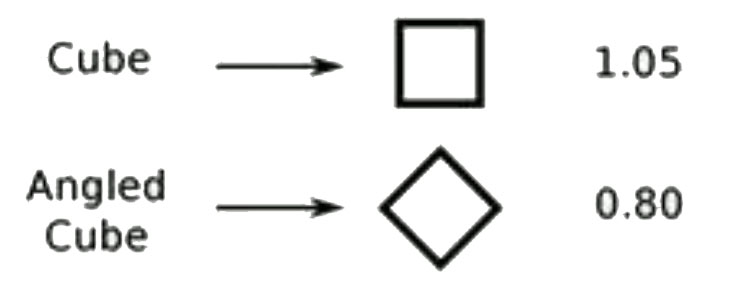
\includegraphics[width=0.8\linewidth]{figures/drag_coef}
			\caption{description needed}
			\label{fig:drag}
		\end{figure}
	\end{minipage}\hfill
	\begin{minipage}[b]{0.49\linewidth}
		\centering
		\begin{figure}[H]
			\centering
			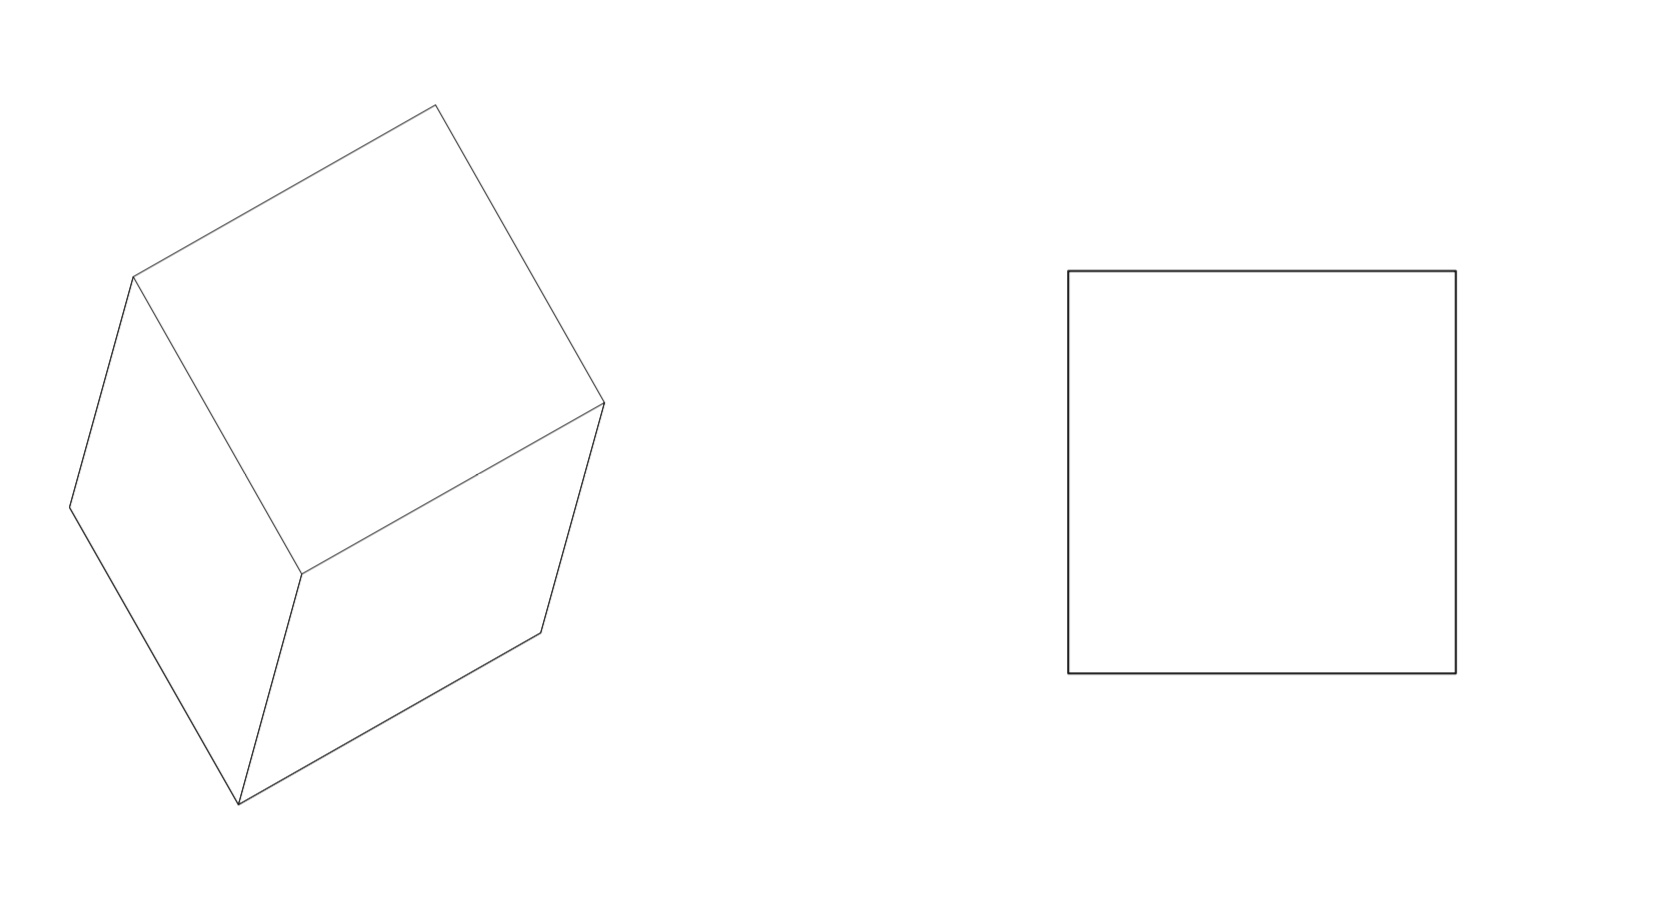
\includegraphics[width=1\linewidth]{figures/a_prep}
			\caption{description needed}
			\label{fig:cub}
		\end{figure}
	\end{minipage}
\end{table}
Therefore, the only parameter that we control is the perpendicular area $A_{\perp}$. The maximum and minimum value of $A_{\perp}$ are represented in \figref{fig:cub}. Thus, the minimum value is the surface of a square of 10cm of dimension ($A_{\perp} = 100cm^2$) and the maximum value is the surface of an hexagone of 10cm of dimension ($A_{\perp} = \frac{3\sqrt{3}}{2} 100cm^2$).
Thus, the drag force can be expressed as the following. 
\[
\vec{F_D} = -u ||\vec{v}|| \vec{v}
\]
with u is the control input and it can take value between $7.27 \cdot 10^{-16}$ and $1.888 \cdot 10^{-15}$.
\subsection{Solar radiation}
Due to low earth orbit flying, the surface of the CubeSat will absorb or reflect the solar radiation, nevertheless, these two situations will alter the CubeSat, which will produce a torque about the satellite center of mass(CoM). 

The torque around CoM is given by:
\begin{flalign}
	N_{rad} = F_{rad} \times R_{CoM}
	\label{eq:tor}
\end{flalign}
where $F_{rad}$  is the solar radiation  and $R_{CoM}$ is the vector from the centre of mass to the geometric centre of radiation

The solar radiation $F_{rad}$ can be expressed as:
\begin{flalign}
	F_{rad} = C_{a} P A
	\label{eq:Pres}
\end{flalign}
where $C_{a}$ is absorption constant of the radiated area and $P$ is the solar flux, while  $A$ is the radiated area
\subsection{$J_2$ gravity perturbation}
A satellite orbiting the Earth encounter multiple perturbing forces. Some of these forces are the atmospheric drag, the gravity gradient, and the solar radiation. The influence of these forces upon the satellite is deemed to be negligible, but one perturbation produced by the oblateness of the Earth is taken into account because will provoke a change in the orientation of the orbit.

The force which the Earth is exerting upon a object outside its sphere is a conservative force and it can be written as follows:
\begin{flalign}
	U(r) = -\frac{\mu}{r}
	\label{eq:Pr}
\end{flalign}
Because the Earth is not a perfect sphere and also its mass distribution is not homogeneous, \eqref{eq:Pr} is rewritten by adding the spherical harmonic expansion to correct the gravitational potential for the Earth:
\begin{flalign}
		U(r) = -\frac{\mu}{r}+ B(r, \phi , \lambda)
	\label{eq:Pr1}
\end{flalign}
where $B(r, \phi, \lambda)$ is the spherical harmonic expansion used to correct the gravitational potential for the Earth's nonsymmetric mass distribution seen in \figref{fig:j2}
\begin{figure}[H]
	\centering
	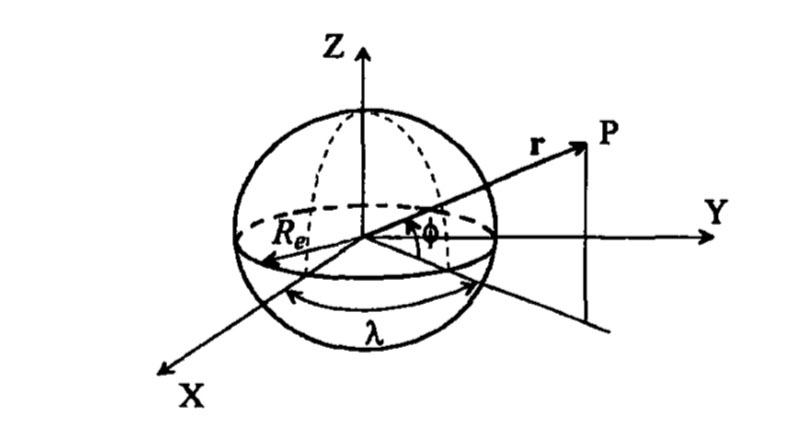
\includegraphics[width=0.6\linewidth]{figures/j2}
	\caption{Coordinates for deriving the external gravitational potential of the Earth }
	\label{fig:j2}
\end{figure} 
In order to solve the problem regarding the oblatness, the gravitational potential of the Earth is extended into series of spherical harmonics: [ref]
\begin{flalign}
	 B(r, \phi , \lambda) = \frac{\mu}{r} \left\{ \sum_{n=2}^{\infty} \left [ \left (\frac{R_e}{r} \right)^{n} J_n P_n sin(\phi)| + \sum_{m=1}^{n} \left (\frac{R_e}{r}\right)^{n} (C_{nm} cos(m\lambda) + S_{nm} sin(m\lambda)) P_{nm} sin(\phi)  \right] \right\} 
	\label{eq:phi2}
\end{flalign}
where $r, \phi , \lambda$ are spherical coordinates and the parameteres from the function are defined as follows: $r$ is the geocentric distance of point $P$, $\phi$ is the geocentric latitude, $\lambda$ is the geographical longitude, $R_e$ is the mean equatorial radius of the Earth, $cos(m\lambda)$ and $sin(m\lambda)$ are harmonics in $\lambda$, $J_{nm}$ are the zonal harmonic coefficients, $J_n$ zonal harmonic coefficients of order 0, $P_{nm} $ associated Legendre polynomial of degree $n$ and order $m$, $P_n$ is Legendre polynomial degree $n$ and order 0, $C_{nm}$ is tesseral harmonic coefficients for $n \neq m$, $S_{nm}$ is sectoral harmonic coefficients for $n =m$

The expression for gravitational potential of the Earth can be approximate as:
\begin{flalign}
   U \approx -\frac{\mu}{r} \left[1 - \sum_{n=2}^{\infty} \left(\frac{R_e}{r}\right)^{n} J_n P_n sin(\phi)  \right ] = \frac{\mu}{r} [U_0 + U_{J_2} + U_{J_3} + ...]
	\label{eq:Pr341}
\end{flalign}
where $U_0$ = -1 and $U_{J_2}$ = $\left(\frac{R_e}{r}\right)^{2} J_2 \frac{1}{2} (3 sin^2 \phi -1) $

The gravitational forces acting on the satellite are obtained from the relation:
\begin{flalign}
	F = -m \nabla U
	\label{eq:Pr3431}
\end{flalign}
and is obtaining the following:
\begin{flalign}
	F_x = -\frac{\partial U}{\partial x} = \mu \left[ -\frac{x}{r^3} + A_{J_2} \left(15 \frac{xz^2}{r^7} - 3\frac{x}{r^5}   \right ) \right ]       \\
		F_y = -\frac{\partial U}{\partial y} = \mu \left[ -\frac{y}{r^3} + A_{J_2} \left(15 \frac{yz^2}{r^7} - 3\frac{y}{r^5}   \right ) \right ]       \\
			F_z = - \frac{\partial U}{\partial z} =  \mu \left[ -\frac{z}{r^3} + A_{J_2} \left(15 \frac{z^3}{r^7} - 3\frac{z}{r^5}   \right )  \right]       
	\label{eq:Pr34331}
\end{flalign}
where $A_{J_2}  = \frac{1}{2} J_2 R_e^2$ and and$R_e$ is the mean radius ofthe earth at the equator
	
\section{State Space Representation}
The state of the system is the vector position and the vecteur velocity in the inertia frame:
\[
\vec{x} = \left[ \begin{array}{c} \vec{p} \\ \vec{v} \end{array} \right]
\]
The equation of (I don't remember the name of the equation xdot = f(x,u) + u) is given by:
\begin{flalign}
\dot{\vec{x}} &= \left[ \begin{array}{c} \dot{\vec{p}} \\ \dot{\vec{v}} \end{array} \right] = \left[ \begin{array}{c} \vec{v} \\ \vec{a} \end{array} \right] \\
 &= \left[ \begin{array}{c} \vec{v} \\ \frac{1}{m_{sat}}(-G\frac{m_{earth} \cdot m_{sat}}{||\vec{p}||^3} \vec{p}) - u ||\vec{v}|| \vec{v} + F_{rad} \end{array} \right] \\
 &= \vec{f(x)} + u \cdot \vec{g(x)} + \vec{\delta(x,t)}
\end{flalign}
with 
\[
\vec{f(x)} = \left[ \begin{array}{c} \vec{v} \\ -G\cdot m_{earth} \frac{\vec{p}}{||\vec{p}||^3} \end{array} \right], \ \vec{g(x)} = \left[ \begin{array}{c} \vec{0} \\ - \frac{1}{m_{sat}}||\vec{v}||\vec{v} \end{array} \right]
\]
and $\vec{\delta(x,t)}$ reprensent the influence all the disturbances.
\section{Relative dynamics}
In order to analyse the distance between two satellites, the relative dynamics is computed. In order to simplify the system. The two will be assumed to stay all over the stay in the same. This assumption has also to be made due to the limitation of the direction of the input control (the drag force). \\
To compute the equations of the motion of one satellite compared to an other one, a new frame is used. The frame is illustrated in the figure\ref{rel_dyn}. The origin is the satellite 1, the axis $\vec{\hat{x}}$ is defined by $\vec{\hat{x}} = \frac{\vec{R}}{R}$ where $\vec{R}$ is the vector from the center of the Earth to the satellite 1, the axis $\vec{\hat{y}}$ is perpendicular to $\vec{\hat{x}}$ and in the plan of motion of the satellites and $\vec{\hat{z}}$ is defined by the right-hand law ($\vec{\hat{z}} = \vec{\hat{x}} \times \vec{\hat{y}}$). \\
\begin{figure}[H]
	\centering
	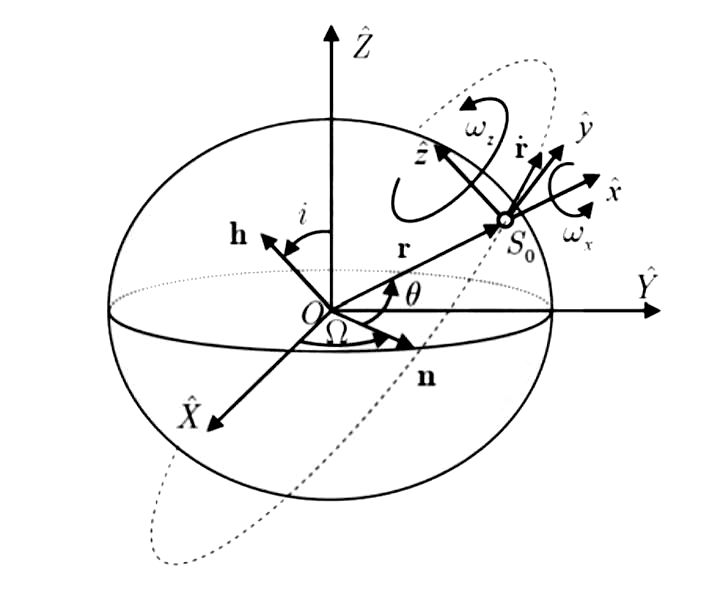
\includegraphics[width=0.6\linewidth]{figures/relativeDynamics}
	\caption{Frame for the relative dynamics}
	\label{fig:rel_dyn}
\end{figure} 
Therefore, the vector position from the earth to the satellite 1 and the satellite 2 can be espressed in this frame:
\begin{flalign}
\vec{p_1} &= R \cdot \vec{\hat{x}} \\
\vec{p_2} &= R \cdot \vec{\hat{x}} + x \cdot \vec{\hat{x}} + y \cdot \vec{\hat{y}} \\
\end{flalign}
The equations of relative motions can ve derived (reference to appendixes):

\chapter{Distance control design}